% Capítulo 3: inserir no início da lista, em três momentos.
\documentclass[border=4pt]{standalone}
\usepackage[utf8]{inputenc}
\usepackage[T1]{fontenc}
% Estilo comum das figuras de listas (incluído pelas figuras dos capítulos 3 e 4).
\usepackage{tikz}
\usetikzlibrary{arrows.meta, positioning, shapes.multipart, calc}
\definecolor{navy}{RGB}{23,45,80}
\definecolor{laranja}{RGB}{250,110,29}
\definecolor{cinzalogo}{RGB}{107,114,126}
\tikzset{
  no/.style={rectangle split, rectangle split horizontal, rectangle split parts=2,
             draw=navy, line width=0.9pt, minimum height=7mm,
             rectangle split part fill={laranja!15, white}, font=\sffamily\small},
  no3/.style={rectangle split, rectangle split horizontal, rectangle split parts=3,
              draw=navy, line width=0.9pt, minimum height=7mm,
              rectangle split part fill={white, laranja!15, white}, font=\sffamily\small},
  seta/.style={-{Stealth[length=2.2mm]}, navy, line width=0.9pt},
  setanova/.style={-{Stealth[length=2.2mm]}, laranja, line width=1.3pt},
  rotulo/.style={font=\sffamily\small\bfseries, text=navy},
  nulo/.style={font=\sffamily\scriptsize, text=cinzalogo},
  passo/.style={font=\sffamily\small, text=cinzalogo, anchor=west},
  legenda/.style={font=\sffamily\scriptsize, text=cinzalogo},
}
% seta que sai do meio da caixa do ponteiro (última parte do nó), na horizontal
\newcommand{\liga}[3][seta]{\draw[#1] ([xshift=-2.3mm]#2.east) -- #3;}

\begin{document}
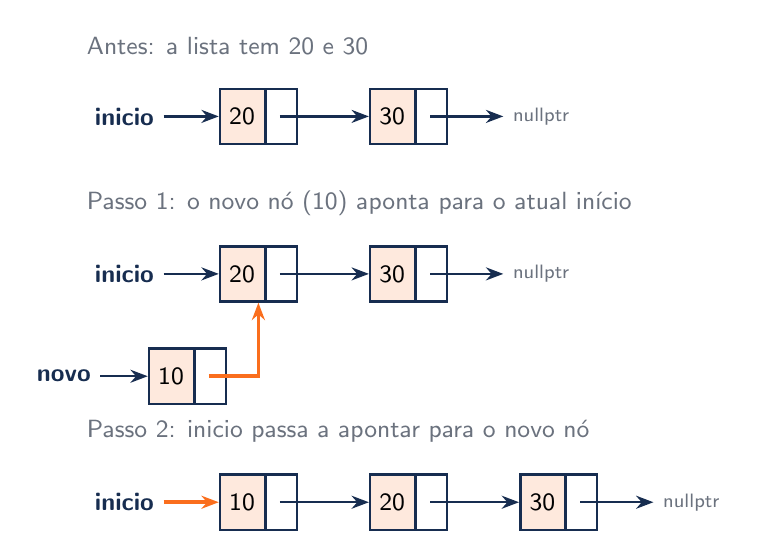
\begin{tikzpicture}[node distance=9mm]
  % antes
  \node[passo] at (-0.6,0.9) {Antes: a lista tem 20 e 30};
  \node[rotulo] (i0) at (0,0) {inicio};
  \node[no, right=7mm of i0] (a0) {20 \nodepart{two} \phantom{x}};
  \node[no, right=of a0] (b0) {30 \nodepart{two} \phantom{x}};
  \node[nulo, right=7mm of b0] (n0) {nullptr};
  \draw[seta] (i0) -- (a0.west);
  \liga{a0}{(b0.west)}
  \liga{b0}{(n0)}

  % passo 1
  \node[passo] at (-0.6,-1.1) {Passo 1: o novo nó (10) aponta para o atual início};
  \node[rotulo] (i1) at (0,-2.0) {inicio};
  \node[no, right=7mm of i1] (a1) {20 \nodepart{two} \phantom{x}};
  \node[no, right=of a1] (b1) {30 \nodepart{two} \phantom{x}};
  \node[nulo, right=7mm of b1] (n1) {nullptr};
  \node[no, below=7mm of i1, xshift=8mm] (x1) {10 \nodepart{two} \phantom{x}};
  \node[rotulo, left=6mm of x1] (nv1) {novo};
  \draw[seta] (i1) -- (a1.west);
  \liga{a1}{(b1.west)}
  \liga{b1}{(n1)}
  \draw[seta] (nv1) -- (x1.west);
  \draw[setanova] ([xshift=-2.3mm]x1.east) -| (a1.south);

  % passo 2
  \node[passo] at (-0.6,-4.0) {Passo 2: inicio passa a apontar para o novo nó};
  \node[rotulo] (i2) at (0,-4.9) {inicio};
  \node[no, right=7mm of i2] (x2) {10 \nodepart{two} \phantom{x}};
  \node[no, right=of x2] (a2) {20 \nodepart{two} \phantom{x}};
  \node[no, right=of a2] (b2) {30 \nodepart{two} \phantom{x}};
  \node[nulo, right=7mm of b2] (n2) {nullptr};
  \draw[setanova] (i2) -- (x2.west);
  \liga{x2}{(a2.west)}
  \liga{a2}{(b2.west)}
  \liga{b2}{(n2)}
\end{tikzpicture}
\end{document}
